\chapter{Numerical Solutions}
\label{sec:Numerical Solutions}

This chapter focuses on the numerical solution of the mentioned systems. It is based on results presented in \cite{NumerikGewöhnlicherDifferentialgleichungen} and \cite{HairerErnst1989Tnso}.

We will first focus on methods used to solve a more general initial value problem of the form:

Find y, such that
\begin{equation}
	\begin{aligned}
		y'(t) &= f(t,y), \quad t \in [t_0, t_l], \\
		y(t_0) &= y_0.
	\end{aligned}
	\label{general numerical problem}
\end{equation}

For this we presume that the function $f(t,y)$ is continuous and Lipschitz-continuous, we can apply the theorem of \emph{Picard-Lindelöf} \protecting{\cite[Satz~1.2.1]{NumerikGewöhnlicherDifferentialgleichungen}}, which states, that for every initial value $y_0$, the initial value problem \eqref{general numerical problem} is uniquely solvable in $[t_0, t_l]$.

In order to obtain an approximation to this unique solution we have to discretize. We first divide the time-intervall $[t_0, t_l]$ into smaller intervals
\begin{displaymath}
	I_{i+1} = [t_i, t_{i+1}] \quad \text{with} \quad i=0,...,N \text{ and } t_0 < t_1 < ... < t_N \leq t_l
\end{displaymath}

and consider approximations $y_m \approx y(t_m)$ on each interval $I_m$ with $m=1,...,N$, see Figure \ref{fig:numerical approximation} for an illustration. We call this a \emph{time-grid} and we call the difference $h_{ij} = t_j - t_i$ with $0 \leq i < j \leq N$ the \emph{step size} from $t_i$ to $t_j$. We will only consider equidistant grids, i.e. $h_{ij} = h$ for all $0 \leq i,j \leq N$. A function defined on such a grid is called a \emph{grid function}.

The grid function $y_h : T \to A$ with the time grid $T=\{t_0, ..., t_N\}$ and the approximated values $A = \{y_0, ..., y_N\}$ is called the \emph{numerical approximation} (of $y$ on the time grid).
\begin{figure}[H]
	\centering
	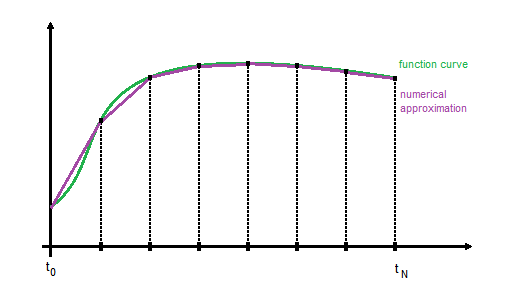
\includegraphics[scale=0.7]{pictures/num_approx.png}
	\caption{approximation of a function}
	\label{fig:numerical approximation}
\end{figure}

%\section{Single Step Methods}
%	The first class of numerical methods we will consider are single step methods. These methods use the previous approximated value $y_j$ and (for implicit methods) also the current approximated value $y_{j+1}$ to determine the current value $y_{j+1}$ through a \emph{procedural function}.
%	
%	\begin{definition}
%		\label{def:single step mehod}
%		A numerical method to approximate a differential equation \ref{general numerical problem} on a time-grid $T =\{t_0,...,t_l\}$ with the intermediate values $y_0,...,y_l$ is called a single step method, if it is of the form
%		\begin{equation}
%			\label{single-step method}
%			y_{j+1} = y_j + h_j \phi(t_j,y_j, y_{j+1},h_j).
%		\end{equation}
%		We call $\phi$ the \emph{procedural function}. If $\phi$ does not depend on $y_{j+1}$, then the method is called \emph{explicit}, otherwise it is called \emph{implicit}.
%	\end{definition}
%
%	\subsection{Consistency, Stability and Convergence}
%	
%	In order to compare different single-step methods we have to define the notions of consistency, stability and convergence. This leads to the definition of the error of the method, its consistency and its convergence. We begin with the definition of the error.
%	
%	\begin{definition}\label{Discretization_Error_SingleStep}
%		Let $y_{m+1}$ be the result of one step of a single step method \eqref{single-step method} with the exact start-vector $y_m = y(t_m)$ then
%		\begin{equation}
%			\label{local discretization error single step}
%			 \delta_{m+1} = \delta(t_m+h) = y(t_{m+1}) - \tilde{y}_{m+1}, \quad m = 0,...,N-1
%		\end{equation}
%		is called the \emph{local discretization error} of the single step method at the point $t_{m+1}$.
%	\end{definition}
%
%	The local error quantifies the error of every step of the method with respect to the exact solution. In most applications the exact solution is not known. Next we consider the consistency.
%
%	\begin{definition}\label{Consistency_SingleStep}
%		A single-step method is called \emph{consistent} if for all initial value problems \eqref{general numerical problem} 
%		\begin{equation}
%			\lim\limits_{h \to 0} \frac{\|\delta(t+h)\|}{h} = 0 \quad \text{for} \quad t_0 \leq t \leq t_l
%		\end{equation}
%		holds.\newline
%		It is called \emph{consistent of order p}, if for a sufficiently smooth function $f$
%		\begin{equation}
%			\|\delta(t+h)\| \leq Ch^{p+1} \quad \text{for all} \quad h \in \mathopen{(} 0,H \mathclose{]} \quad \text{and} \quad t_0 \leq t \leq t_l - h
%		\end{equation}
%		holds with $C$ independent of $h$.
%	\end{definition}
%
%	Consistency aims to give insight in how similar the problem \eqref{single-step method} that the numerical method solves is to the real problem \eqref{general numerical problem}. Finally we consider convergence of a single step method \ref{def:single step mehod}.
%
%	\begin{definition}\label{Convergence_SingleStep}
%		A single-step method is called \emph{convergent}, if for all initial value problems \eqref{general numerical problem} for the \emph{global discretization error}
%		\begin{displaymath}
%			e_m = y(t_m)-y_m
%		\end{displaymath}
%		holds that
%		\begin{displaymath}
%			\max\limits_{m}\|e_m\| \to 0 \quad \text{for} \quad h_{max} \to 0.
%		\end{displaymath}
%		The single-step method is called to have the \emph{convergence order} $p$, if
%		\begin{displaymath}
%			\max\limits_{m} \|e_m\| \leq C h_{max}^p \quad \text{for} \quad h_{max} \in \mathopen{(} 0,H \mathclose{]} \quad \text{with} \quad t_0 \leq t_m \leq t_l
%		\end{displaymath}
%		with the constant $C$ not dependent on the step size $h$.
%	\end{definition}
%
%	As the name suggestes convergence tries to quantify how far off a numerical solution is from the real solution of a system. A very interesting result follows if we additionally require the single-step method to be stable.
%	
%	\begin{definition}\label{Discrete_Stability_SingleStep - lecture notes for numpdgl}
%		A single-step method is called \emph{(discretely) stable} if for grid-functions $y_h$ and $\tilde{y}_h$ with
%		\begin{align}
%			y_{i+1} &= y_i + h \phi(t_i, y_i), \\
%			\tilde{y}_{i+1} &=  \tilde{y}_i + h [\phi(t_i, \tilde{y}_i) + \theta_i],
%		\end{align}
%		and perturbations $\theta_i = \theta_h(t_i)$ of the right side as well as a bounded perturbation in the initial-values $y_0 - \tilde{y}_0$ the error is bounded by
%		\begin{displaymath}
%			\|y_h - \tilde{y}_h\|_{\infty,h} \leq C (\|y_0 - \tilde{y}_0\|_{l^2} + \|\theta_h\|_{\infty,h})
%		\end{displaymath}
%		with a constant $C$ which is not dependent on $h$. The norm $\|.\|_{\infty,h}$ denotes the maximum norm over the time-grid, i.e. for a function $b: T={t_0,...,t_N} \to \mathbb{R}^d$ we have $\|b\|_{\infty,h} = \max\limits_{t \in T}\|b(t)\|$, $\|b\|$ is the euclidean norm.
%	\end{definition}
%	
%	For single-step methods which are consistent and stable we obtain the following convergence theorem.
%	
%	\begin{theorem}[Lax-Richtmyer]\label{Lax-Richtmyer}
%		A consistent (with order $p$) and discretely stable single-step method is convergent (with order $p$).
%	\end{theorem}
%	
%	This theorem is due to Lax and Richtmyer. The converse of this statement is also true. 
%
%	\subsection{Further stability properties}
%		from numpdgl skript \\
%		In this section we consider as a model problem the Dahlquist equation, i.e. find $y:\mathbb{R} \to \mathbb{C}$ such that
%		\begin{align}
%			y' &= \lambda y, \quad t > 0 \\
%			y(0) &= y_0
%		\end{align}
%		with $\lambda \in \mathbb{C}$ and $y_0 \in \mathbb{C}$ fixed.
%		
%		\begin{definition}
%			\begin{enumerate}
%				\item 
%				If a single-step method can be written in the form
%				\begin{equation}
%					y_{i+1} = R(z) \ y_i, \quad z:= h \lambda
%				\end{equation}
%				then we call $R: \mathbb{C} \to \mathbb{C}$ the \emph{stability function} of the single-step method.
%				\item 
%				The set
%				\begin{equation}
%					S := \{z \in \mathbb{C} : |R(z)| \leq 1\}
%				\end{equation}
%				is called the \emph{region of stability} of the method.
%				\item 
%				A single-step method is called
%				\begin{itemize}
%					\item \emph{0-stable}, if $0 \in S$.
%					\item \emph{A-stable}, if $\mathbb{C}^- \subset S$, where $\mathbb{C}^- = \{x \in \mathbb{C} : Re(x) \leq 0 \}$
%					\item \emph{L-stable}, if $R(z) \to 0$ for $Re(z) \to -\infty$.
%				\end{itemize}
%			\end{enumerate}
%		\end{definition}

	%\subsection{Runge-Kutta Methods}
	%	A very prevalent family of numerical single-step methods are the \emph{Runge-Kutta} methods. 
		
		%\begin{figure}
		%	\centering
		%	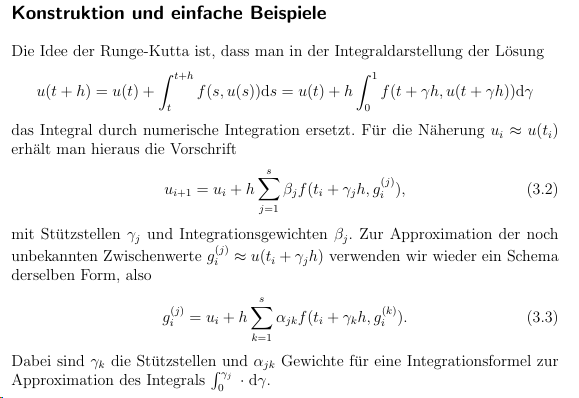
\includegraphics[width=0.7\linewidth]{screenshot026}
		%	\caption{}
		%	\label{fig:screenshot026}
		%\end{figure}
		
	%	\begin{definition}
	%		Let $s \in \mathbb{N}$. A single-step method of the form
	%		\begin{align}
	%			y_{m+1} = y_m + h \sum_{i=1}^{s} b_i f(t_m + c_ih, y_{m+1}^{(i)}) \\ 
	%			y_{m+1}^{(i)} = y_m +  \sum_{j=1}^{s} a_{ij} f(t_m + c_jh, y_{m+1}^{(j)})
	%		\end{align}
	%		is called a \emph{Runge-Kutta Method} with $s$ steps.
	%	\end{definition}
		
	%	We usually collect the coefficients into the vectors and matrices $c=(c_1, ...,c_s)$, $A = (a_{ij})_{ij}$ and $b=(b_1, ..., b_s)$.
		
	%	If $A$ is a strictly lower triangle matrix, this means for all $j \geq i$ holds $a_{ij} = 0$ then the Runge-Kutta method is explicit, otherwise it is implicit. In general implicit Runge-Kutta methods might need more computational effort because to calculate $y_m^{(i)}$ a nonlinear system of equations has to be solved. But in contrast those methods can also lead to very good stability characteristics.
		
	%	\begin{lemma}\cite{NumerikGewöhnlicherDifferentialgleichungen}
	%		A Runge-Kutta mehtod is consistent, if and only if
	%		\begin{displaymath}
	%			\sum_{i=1}^{s} b_i = 1
	%		\end{displaymath}
	%	\end{lemma}
	
	%	The coefficients of a Runge-Kutta method are usually represented in the \emph{Butchertableau}, which was introduced by John C. Butcher and has the following form.
		
	%	\begin{displaymath}
	%		\begin{array}{c|ccc}
	%			c_1 & a_{11} & \dots & a_{1s} \\
	%			\vdots & \vdots & & \vdots \\
	%			c_s & a_{s1} & \dots & a_{ss} \\
	%			\hline
	%			 & b_1 & \dots & b_s
	%		\end{array}
	%		\qquad
	%		\text{of in matrix form}
	%		\qquad
	%		\begin{array}{c|c}
	%			c & A \\
	%			\hline
	%			 & b
	%		\end{array}
	%	\end{displaymath}
	
	%	Their stability can directly be derived from the butcher tableau. The stability function of an arbitrary m-stage Runge-Kutta method has the form
	%	\begin{displaymath}
	%		R(z) = 1+zb^\top (I_m-zA)^{-1}e
	%	\end{displaymath}
	
	%	where $e = (1,...,1)$.
		
	%	\textbf{Remark:} The trapezoidal rule is a widely used Runge-Kutta method which we can also consider as a multistep-method. It will be discussed later on.
	
			
\section{Multistep Methods}
	\label{sec:multistep methods}
	
	In this thesis we will only consider the class of \emph{linear multistep methods} (LMSM). This chapter is in large parts based on \cite{NumerikGewöhnlicherDifferentialgleichungen}. These methods use multiple previously approximated values $y_{m+l}$ at the gridpooints  $t_{m+l}, \quad l=0,1,...,k-1$ to approximate the current value $y_{m+k}$ at $t_{m+k}$. The definition for such a method is given in \ref{def:multi step method}
	
	\begin{definition}
		\label{def:multi step method}
		For given $\alpha_0, ..., \alpha_k$ and $\beta_0, ..., \beta_k$ the iteration rule
		\begin{equation}
			\label{linear-multistep-method}
			\sum_{l=0}^{k} \alpha_l y_{m+l} = h \sum_{l=0}^{k} \beta_l f(t_{m+l}, y_{m+l}), \quad m=0,1,...,N-k
		\end{equation}
		is called a \emph{linear multistep method} (linear k-step method). It is always assumed that $\alpha_k \neq 0$ and $|\alpha_0| + |\beta_k| > 0$. If $\beta_k=0$ holds, then the method is called \emph{explicit}, otherwise it is called \emph{implicit}.
	\end{definition}
	
	The calculation of approximations using a multistep method consists of two phases:
	\begin{enumerate}
		\item In the \emph{starting-phase} approximations $y_1,...,y_{k-1}$ for the first $k-1$ gridpoints $t_l = t_0+l\ h, l=1,...,k-1$ have to be calculated. For example we can use a single-step method or a multi-step method with fewer steps.
		
		\item  In the \emph{run-phase} the multi-step formula is used to determine new approximations $u_{m+k}$ for the gridpoint $t_{m+k}$
	\end{enumerate}
	

	
	\subsection{Consistency, Stability and Convergence}
	
	In order to compare different multistep methods we have to introduce the notions of error, consistency, stability and convergence. We begin with the definition of the error.
	\begin{definition}
		Let $y_{m+k}$ be the result of one step of the multi-step method \eqref{linear-multistep-method} with the start-values given as the evaluations of the exact solution $y_{m+l} = y(t_{m+l})$ at $0 \leq l < k$. This means
		\begin{displaymath}
			\alpha_k y_{m+k} = \sum_{l=0}^{k-1} \left( h \beta_l f(t_{m+l}, y(t_{m+l})) - \alpha_l y(t_{m+l}) \right) + h \beta_k f(t_{m+k}, y_{m+k}) .
		\end{displaymath}
		Then
		\begin{displaymath}
			\delta_{m+k} = y(t_{m+k}) - y_{m+k}, \quad m=0,1,...,N-k
		\end{displaymath}
		is called the \emph{local discretization error} (local error) of the linear multi-step method \eqref{linear-multistep-method} at the point $t_{m+k}$.
	\end{definition}
	
	If we assign the difference operator
	\begin{equation}
		L[y(t),h] = \sum_{l=0}^{k} \left( \alpha_l y(t+lh) - h \beta_l y'(t+lh) \right)
	\end{equation}
	to the linear mutli-step method, we gain the following definition for consistency of such a methods.
	
	%%%%%%%%%%%%%%%%%%%%%%%%%%%%%%%%%%%%%%%%%%%%%%%%%%%%%%%%%%%%%%%pagebreak%%%%%%%%%%%%%%%%%%%%%%%%%%%%%%%%%%%%%%%%%%%%%%%%%%%%%%%%%%%%%%%%%%%%%%%%%%%%%%%%
	\newpage
	%%%%%%%%%%%%%%%%%%%%%%%%%%%%%%%%%%%%%%%%%%%%%%%%%%%%%%%%%%%%%%%%%%%%%%%%%%%%%%%%%%%%%%%%%%%%%%%%%%%%%%%%%%%%%%%%%%%%%%%%%%%%%%%%%%%%%%%%%%%%%%%%%%%%%%%%
	
	\begin{definition}
		A linear multi-step method is called %\emph{preconsistent} if for all functions $y(t) \in C^1[t_0,t_l]$
%		\begin{displaymath}
%			\lim\limits_{h \to 0} L[y(t),h]=0
%		\end{displaymath}
%		holds. 
%		It is called 
		\emph{consistent}, if for all functions $y(t) \in C^2([t_0,t_l])$
		\begin{displaymath}
			\lim\limits_{h \to 0} \frac{1}{h} L[y(t),h] = 0
		\end{displaymath}
		holds. It is called \emph{consistency with order p}, if for all functions $y(t) \in C^{p+1}[t_0, t_l]$
		\begin{displaymath}
			L[y(t),h] = \mathcal{O}(h^{p+1}) \quad \text{for} \quad h \to 0
		\end{displaymath}
		holds.
	\end{definition}

	From the generating polynomials \eqref{eq:generating polynomials multistep method} we can derive simple consistency conditions, i.e.
	\begin{displaymath}
		\rho(1) = 0 \quad \text{and} \quad \rho'(1) = \sigma(1).
	\end{displaymath}

	Next we also need convergence of such methods.
	
	\begin{definition} \label{def: LMSM convergence}
		We say that a linear multi-step method is convergent, if for a solution $y$ of the problem and a vector $(y_j)_{j=0}^k$ created by an LMSM , we have that
		\begin{displaymath}
			\lim\limits_{h \to \infty} \max_{0 \leq j \leq k} ||y(t_j) - y_j|| = 0.
		\end{displaymath}
		If for $p \in \mathbb{N}$ and a constant $C$ not dependent on the step size $h$ we have
		\begin{displaymath}
			\max_{0 \leq j \leq k} ||y(t_j) - y_j|| \leq Ch^p,
		\end{displaymath}
		then we call the LMSM \emph{convergent with order $p$}.
	\end{definition}
	
	%\begin{figure}
	%	\centering
	%	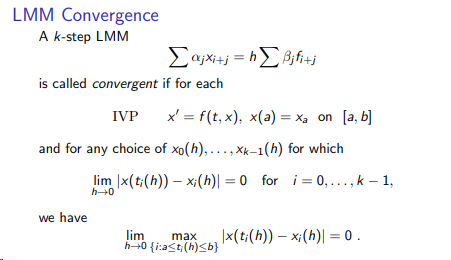
\includegraphics[width=0.7\linewidth]{screenshot025}
	%	\caption{}
	%	\label{fig:screenshot025}
	%\end{figure}
	
	The notion of stability output continuously dependent on input. Thus we consider two different inputs for this definition and compare their outputs.
	
	%%%%%%%%%%%%%%%%%%%%%%%%%%%%%%%%%%%%%%%%%%%%%%%%%%%%%%%%%%%%%%%pagebreak%%%%%%%%%%%%%%%%%%%%%%%%%%%%%%%%%%%%%%%%%%%%%%%%%%%%%%%%%%%%%%%%%%%%%%%%%%%%%%%%
	\newpage
	%%%%%%%%%%%%%%%%%%%%%%%%%%%%%%%%%%%%%%%%%%%%%%%%%%%%%%%%%%%%%%%%%%%%%%%%%%%%%%%%%%%%%%%%%%%%%%%%%%%%%%%%%%%%%%%%%%%%%%%%%%%%%%%%%%%%%%%%%%%%%%%%%%%%%%%%
	
	\begin{definition} \label{discrete stability LMSM}
		A linear multi-step method is called (discretely) stable, if for solution vectors $(y_l)_{l=0}^k$ and $(\tilde{y}_l)_{l=0}^k$ of
		\begin{align}
			\sum_{l=0}^{k} \alpha_l y_{m+l} &= h \sum_{l=0}^{k} \beta_l f(t_{m+l}, y_{m+l}), \\
			\sum_{l=0}^{k} \alpha_l \tilde{y}_{m+l} &= h \sum_{l=0}^{k} \beta_l f(t_{m+l}, \tilde{y}_{m+l}) + h\theta_m,
		\end{align} 
		where and bounded initial values $y_j$, $\tilde{y}_j$ for $j \in {0,...,k}$, we have that
		\begin{displaymath}
			\max_{t_0 \leq t_n \leq T} ||y_n - \tilde{y}_n|| \leq C \sum_{j=0}^{k-1} ||y_j - \tilde{y}_j|| + \max_{t_0 \leq t_n \leq T} ||\theta_n||.
		\end{displaymath}
	\end{definition}
	
%	\begin{definition}
%		A linear multi-step method is called \emph{zero-stable} if all solutions of the difference equation
%		\begin{displaymath}
%			\sum_{l=0}^{k} \alpha_l u_{m+l} = 0
%		\end{displaymath}
%		are bounded.
%	\end{definition}
	
%	\textbf{Lax-Richtmyer}
	
%	\begin{theorem}
%		A linear multi-step method is zero-stable, if and only if the polynomial $\rho(x)$ fullfills the ``root-condition'', this means:
%		\begin{enumerate}
%			\item All roots $\bar{x}$ of $\rho(x)$ are within the unit-circle $|\bar{x}| \leq$ in the complex plane.
%			\item All roots $\bar{x}$ with $|x| = 1$ are singular.
%		\end{enumerate}
%	\end{theorem}
	
%	\begin{theorem}%[DAE lecture]
%		A linear multistep method is stable if and only if it is zero-stable.
%	\end{theorem}
	
	%\textbf{from circuit book below, above from modelling book}
	
	\subsection{Further stability properties}
	
	In this section we consider again the Dahlquist test problem as a model problem, i.e. find $y:\mathbb{R} \to \mathbb{C}$ such that
	\begin{align}
		y' &= \lambda y, \quad t > 0 \\
		y(0) &= y_0
	\end{align}
	with $\lambda \in \mathbb{C}$ and $y_0 \in \mathbb{C}$ fixed.\\
	
	%Asessment for stiff equations lt wikipedia (LMSM)
	
	Thus the resulting linear multistep method is of the form
	\begin{align*}
		\sum_{l=0}^{k} \alpha_l y_{n+l} = h \sum_{l=0}^{k} \beta_l \lambda y_{n+l} \\
		\iff \sum_{l=0}^{k}  [\alpha_l - h \beta_l \lambda] y_{n+l} = 0
	\end{align*}
	
	%in numerik book auf seite 326
	
	We define the two polynomials $\rho(x)$ and $\sigma(x)$ to ...
	For theoretical analysis of the multi-step methods we consider the generating polynomials of a multistep method.
	\begin{equation}
		\label{eq:generating polynomials multistep method}
		\rho(x) := \sum_{l=0}^{k} \alpha_l x^l
		\qquad \text{and} \qquad
		\sigma(x) := \sum_{l=0}^{k} \beta_l x^l
	\end{equation}
	
	
	Using this we define the following important stability notions.
	\begin{definition}
		\begin{enumerate}
			\item 
			The set
			\begin{equation}
				\begin{aligned}
					S := \{z \in \mathbb{C} : \rho(\xi) - z \sigma(\xi) = 0 \implies \xi \in \mathbb{C} \text{ and } |\xi| \leq 1. \\
					\text{ If $\xi$ has multiplicity greater than $1$, then } |\xi| < 1\}
				\end{aligned}
			\end{equation}
			is called the region of stability of the method.
			\item 
			A linear multistep method is called
			\begin{itemize}
				\item \emph{0-stable}, if $0 \in S$.
				\item stable in the point $z \in \mathbb{C}$, if $z \in S$.
				\item \emph{$A(\alpha)$-stable}, if it is stable in all $z$ that lie within the set $\{z \in \mathbb{C}^- : |arg(z)-\pi| \leq \alpha\}$ for $\alpha \in (0, \frac{\pi}{2})$.		 
			\end{itemize}
		\end{enumerate}
	\end{definition}
	
	%seite 314 im buch numerik 
	
	\begin{figure}[H]
		\centering
		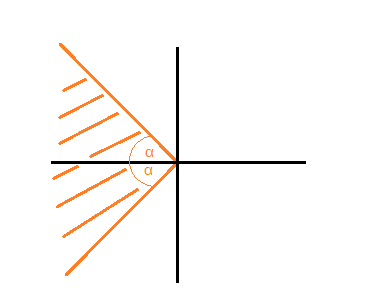
\includegraphics[width=0.3\linewidth]{pictures/A_alpha_stability.png}
		\caption{$A(\alpha)$ stability for $\alpha = \frac{\pi}{4}$}
		\label{fig:A of alpha stability}
	\end{figure}
	
	%following from numerik buch seite 134
	\begin{theorem}[\protecting{\cite[Satz~4.2.10]{NumerikGewöhnlicherDifferentialgleichungen}}]
		\label{th: null-stbaility and consistence is convergence}
		Let $f(t,y)$ be sufficiently smooth and the linear multi-step method be zero-stable and consistent of order $p$, then it is also convergent of order $p$.
	\end{theorem}
	
	%equivalent to lax richtmyer in single step because for lmsm zero stable = stable
	
\section{Implicit linear multistep formulas}
In this chapter we discuss three different linear multistep methods. Whereas the trapezoidal rule and the implicit midpoint rule (or Gauss with one stage) really only use one timestep to approximate the next value and might thus be considered as \emph{singlestep} methods, the Backward-Differentiation-Fomulas with $k$ stages (BDF-k) really use $k$ steps and thus are ``true'' multistep methods.
We will see that the BDF-k methods as well as the trapezoidal rule are preferably used over the implicit midpoint rule due to their advantageous behaviour when applied to differential algebraic equations. Examples are discussed in \ref{sec: numerical examples}. For more detailed analysis of the mentioned methods we refer to \cite{NumerikGewöhnlicherDifferentialgleichungen} and \cite{HairerErnst1989Tnso}.
%Our assumption that we only consider network equations arising from networks consisting of RLC components as well as controlled sources which keep the index between 1 and 2 still holds.

%We consider the equations in charge/flux oriented formulation introduced in section \ref{sec:charge flux oriented formulation}
%\begin{align*}
%	0 &=
%	\underbrace{ 
%	\left( \begin{matrix}
%		A_c & 0 \\
%		0 & I \\
%		0 & 0
%	\end{matrix} \right)}_{=:A}
%	\underbrace{
%	\left( \begin{matrix}
%		q' \\
%		\phi'
%	\end{matrix} \right)}_{=:y'}
%	+
%	\underbrace{
%	\left( \begin{matrix}
%		A_R r(A_R^\top u,t) + A_L i_L + A_V i_V + A_I i(u, i_L, i_V, t) \\
%		- A_L^\top u \\
%		v(u, i_L, i_V, t) - A_V^\top u
%	\end{matrix} \right)}_{=:f(x,t)}, \\
%	\underbrace{
%	\left( \begin{matrix}
%		q \\
%		\phi 
%	\end{matrix} \right)}_{=:y} 
%	&=
%	\underbrace{
%	\left( \begin{matrix}
%		q_C(A_C^\top u) \\
%		\phi_L(i_L) 
%	\end{matrix} \right)}_{=:g(x,t)},
%\end{align*}
%
%or simply
%\begin{align*}
%	0 &= F(y'(t), x(t), t) :=A y'(t) + f(x(t),t), \\
%	0 &= y(t) - g(x(t)).
%\end{align*}
%with the unknowns $x:=(u, i_L, i_V)^\top$.

In Section \ref{sec:multistep methods} we did already talk about the starting- and the run-phase of a multistep method. However, we left out one important aspect of the starting phase. Recall that in the starting phase we calculate the first $k-1$ steps using a method with fewer stages than the method we want to use ultimately. This also means that this method might be of lower order than the final method. To achieve the desired convergence rates it is thus also important to compute these initial steps appropriately, i.e. the method with which these initial steps are calculated has to also be of the desired order with respect to the \emph{final} step size $h$. (In applications this can mean that we calculate the initial steps with methods of lower order, but compensate by using a smaller step-size)

\subsection{BDF-k methods}
	\label{sec:BDFk}

	The Backward-Differentiation-Formulas with $k$ stages (or short \emph{BDF-k methods}) are constructed, such that they are $A(\alpha)$-stable with the largest possible angle $\alpha$. We will not go into detail about their construction, for this we again refer to \protecting{\cite[chapter~9.2]{NumerikGewöhnlicherDifferentialgleichungen}}

	We will not give a deeper look into their construction but will only state their properties. BDF schemes are appealing because they save function evaluations as much as possible.
	
	The BDF-k methods have the general form
	\begin{equation}
		\sum_{k=0}^{s} \alpha_k y_{n+k} = h \beta f(t_{n+s}, y_{n+s}).
	\end{equation}

	Due to the construction of the method, which is not built around conserving zero-stability, the method is not zero-stabel for all $k \in \mathbb{N}$. It turns out that it is only zero-stable for $k \leq 6$, \protecting{\cite[page~325]{NumerikGewöhnlicherDifferentialgleichungen}}. However in practice, methods with order greater than $3$ are rarely used because of their stability properties, as the stability-region shrinks with increasing order.
	
	The BDF or BDF-k formulas for $k=1,...,3$ have the following form %or till 6
	\begin{align*}
		k = 1 &: h f_{m+1} = y_{m+1} - y_m \\
		k = 2 &: h f_{m+2} = \frac{1}{2} (3 y_{m+2} - 4 y_{m+1} + y_m) \\
		k = 3 &: h f_{m+3} = \frac{1}{6} (11 y_{m+3} - 18 y_{m+2} + 9 y_{m+1} - 2 y_m) %\\
%		k = 4 &: h f_{m+4} = \frac{1}{12} (25 u_{m+4} - 48 u_{m+3} + 36 u_{m+2} - 16 u_{m+1} + 3 u_m) \\
%		k = 5 &: h f_{m+5} = \frac{1}{260} (137 u_{m+5} - 300 u_{m+4} + 300 u_{m+3} - 200 u_{m+2} +75 u_{m+1} -12 u_m) \\
%		k = 6 &: h f_{m+6} = \frac{1}{60} (147 u_{m+6} - 360 u_{m+5} + 450 u_{m+4} - 400 u_{m+3} + 225 u_{m+2} - 72 u_{m+1} + 10 u_m)
	\end{align*}
		
	As already mentioned BDF-k methods are not A-stable, but $A(\alpha)$ stable. In Figure \ref{fig:bdf-k stability regions} the stability regions for $k=1,2,3$ are depicted in cyan. Note that the zero-point is contained withing the stability regions.
		
	\begin{figure}[H]
		\centering
		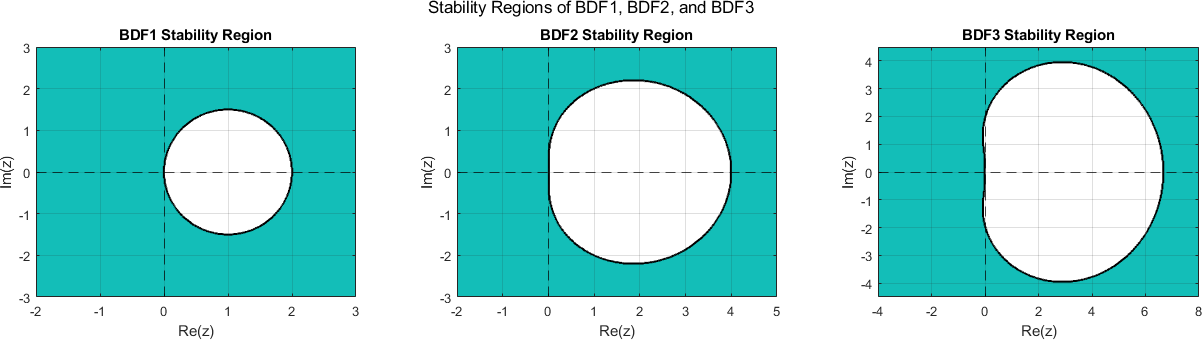
\includegraphics[width=1\linewidth]{pictures/bdf_stability_regions.png}
		\caption{stability regions of BDF-k methods for $k=1,2,3$ (cyan)}
		\label{fig:bdf-k stability regions}
	\end{figure}

	The order of consistency of this family of multi-step methods is given by the following theorem
	
	\begin{theorem}[\protecting{\cite[Satz~9.2.1]{NumerikGewöhnlicherDifferentialgleichungen}}]
		\label{th: BDK-k consistency}
		The BDF-k methods have consistency order $p=k$.
	\end{theorem}
	
	Due to Theorem \ref{th: null-stbaility and consistence is convergence} and the fact that BDF-k methods with $k \leq 6$  are $0$-stable as well as Theorem \ref{th: BDK-k consistency} we immediately gain the following corollary.
	
	\begin{corollary}[Convergence rate]
		The BDF-k methods with $k \leq 6$ are convergent with order$k$
	\end{corollary}
	
	%Seite 106 numerik - schrittweite für startwerte bei bdf3 kleiner für kleineren fehler, halbieren, vierteln, achteln whatever
	
\subsection{Trapezoidal rule}
	\label{sec:Trapezoidal}
	
	By approximating the area under a curve $f(x)$ on a short interval $[a,b]$ as a trapezoid, 
	\begin{displaymath}
		\int_{a}^{b} f(x) dx \approx (b-a)\frac{1}{2} (f(a)+f(b)),
	\end{displaymath}
	
	we can construct a numerical method for integrating a function. This method is called the trapezoidal rule, formally it has the iteration rule
	\begin{displaymath}
		y_{n+1} = y_n +\frac{h}{2}[f(t_n,y_n) + f(t_{n+1}, y_{n+1})].
	\end{displaymath}
	
	%	This iteration rule can also be formulated using the butcher tableau	
%	\begin{displaymath}
%		\begin{array}{c|cc}
%			0 & 0 & 0 \\
%			1 & \frac{1}{2} & \frac{1}{2} \\
%			\hline
%			& \frac{1}{2} & \frac{1}{2}
%		\end{array}
%	\end{displaymath}
	
	The trapezoidal rule has convergence order $p=2$ for our applications. For details see \cite{HairerErnst1989Tnso}, where more general the general form of the trapezoidal rule, namely the Lobatto~\RomanNumeralCaps{3}-A methods amongst other methods are discussed.
	
	Due to the fact that the trapezoidal rule is A-stabe  (\cite{ModellingAndDiscretizationOfCircuitProblems}) and of order $p=2$, it can be considered as a natural alternative to the BDF-2 method.
	
	%order p=2 because it is a special case of Lobatto 3 A with s=2, thus all the index cases just lead to p=2
	
\subsection{Gauss Method with one stage}
	\label{sec:Gauss1}

	We have already seen that the results for the BDF-k methods as well as for the trapezoidal rule are relatively straight forward. But this is not always the case, many numerical methods can cause problems when applied to DAEs, see also \cite{HairerErnst1989Tnso}. To illustrate this we will have a look at the Gauss method with one stages, also called the implicit midpoint rule, i.e.
	\begin{displaymath}
		y_{n+1} = y_n + h f(t_n + \frac{h}{2}, \frac{y_n + y_{n+1}}{2})
	\end{displaymath}

	Applied to ordinary differential equations, this method yields a convergence order of $p=2$ \protecting{\cite[chapter~8.1.2]{NumerikGewöhnlicherDifferentialgleichungen}}. For the special case of differential algebraic equations this does not hold true. Here we may observe lower convergence rates, especially in the algebraic variable. The convergence orders for this method are also different, if the amount of stages is even or odd. We say that this method is \emph{not stiffly accurate}. Table \ref{tab:convergence order Gauss} displays the according convergence orders.
	
	\begin{table}[H]
		\centering
		\begin{tabular}{ | c | c c | c c |}
			\hline
			\multirow{2}*{number of stages $s$} & \multicolumn{2}{c |}{index $\nu = 1$} & \multicolumn{2}{ c |}{index $\nu = 2$} \\
			 & differential & algebraic & differential & algebraic \\
			 \hline
			 even & \multirow{2}*{$2s$} & $s+1$ & $s+1$ & $s-1$ \\
			 odd & & $s$ & $s$ & $s-2$ \\
			 \hline
		\end{tabular}
		\caption{Convergence order for Gauss method.}
		\label{tab:convergence order Gauss}
	\end{table}
	
\section{Numerical Examples}
	
	\label{sec: numerical examples}
	In this section we will apply the trapezoidal rule, the BDF-k method and the implicit midpoint rule, discussed in Section \ref{sec:BDFk}, Section \ref{sec:Trapezoidal} and Section \ref{sec:Gauss1} to our three examples. We will also discuss the discretization error in the solution and compute appropriate consistant inital values for our problems. The code used is provided in Section \ref{sec:Code listings}.
	

\subsection{BDF-k Method and Trapezoidal Rule}	

	We will start by applying the ``well-behaving'' methods to our examples.
	
\begin{example1}[Numerical computation]
	We again consider the charging of a capacitor, depicted in the schematics in Figure \ref{fig:charging capacitor}.
	
	\begin{figure}[H]
		\centering
		\begin{minipage}{.5\textwidth}
			\centering
			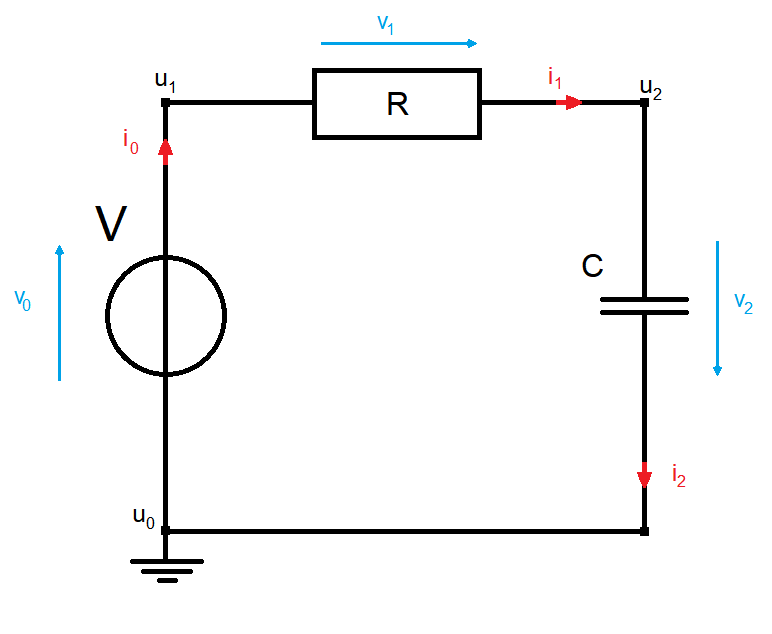
\includegraphics[width=\linewidth]{pictures/Example1_simple_p2.png}
			\caption{charging capacitor with series resistor and voltage source}
			\label{fig:charging capacitor}
		\end{minipage}%
		\begin{minipage}{.5\textwidth}
			\centering
			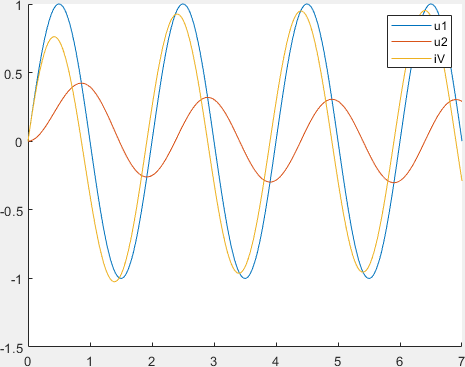
\includegraphics[width=\linewidth]{pictures/exact_solution_ex1.png}
			\caption{Exact solution for example 1.}
			\label{fig: Exact solution for example 1}
		\end{minipage}
	\end{figure}
	
	For testing we set the resistance to $R=1$ and the capacitance to $C=1$. In our case we let the  voltage source supply a voltage of the form $v_{src} = sin(\pi t)$. The resulting MNA-system for this example reads
	\begin{equation}
		\label{eq:MNA-system of chargin capacitor with explicit values}
		\begin{pmatrix}
			0 & 0 & 0 \\
			0 & 1 & 0 \\
			0 & 0 & 0
		\end{pmatrix}
		*
		\begin{pmatrix}
			u_,' \\
			u_2' \\
			i_0'
		\end{pmatrix}
		+
		\begin{pmatrix}
			1 & 1 & -1 \\
			1 & 1 & 0 \\
			1 & 0 & 0 
		\end{pmatrix}
		*
		\begin{pmatrix}
			u_1 \\
			u_2 \\
			i_0
		\end{pmatrix}
		=
		\begin{pmatrix}
			0 \\
			0 \\
			-sin(\pi t)
		\end{pmatrix}.
	\end{equation}
		
	We expect the resulting potentials and currents to be of the form seen in Figure \ref{fig: Exact solution for example 1}.

	The resulting errors for our numerical tests are displayed in table \ref{tab:num results ex1}, we omit $u_1$ since it just equals $-v_{src}$ and thus produces no interesting error results. The reported errors are computed using $err(y) = \max\limits_{0 \leq n \leq N} | y(t_n) - y_n |$ where $y_n$ denotes the numerical approximation and $y(t_n)$ denoted the exact solution at the time-step $t_n$. 
	
	\begin{table}[H]
		\resizebox*{\textwidth}{!}{%
			\csvreader[tabular= | c || c c | c c | c c | c c |,
			table head = \hline h & \multicolumn{2}{c|}{k = 1} & \multicolumn{2}{c|}{k = 2} & \multicolumn{2}{c|}{k = 3} & \multicolumn{2}{c|}{trapezoidal}\\
			& $err(u_2)$ & $err(i_V)$ & $err(u_2)$ & $err(i_V)$ & $err(u_2)$ & $err(i_V)$ & $err(u_2)$ & $err(i_V)$  \\
			\hline,
			late after line=\\\hline]
			{../Matlab/err_ex1.csv}{h=\h, oneu=\oneu, oneueoc=\oneueoc, oneuu=\oneuu, oneuueoc=\oneuueoc, onei=\onei, oneieoc=\oneieoc, twou=\twou, twoueoc=\twoueoc, twouu=\twouu, twouueoc=\twouueoc, twoi=\twoi, twoieoc=\twoieoc, threeu=\threeu, threeueoc=\threeueoc, threeuu=\threeuu, threeuueoc=\threeuueoc, threei=\threei, threeieoc=\threeieoc, trapu=\trapu, trapueoc=\trapueoc, trapuu=\trapuu, trapuueoc=\trapuueoc, trapil=\trapil, trapileoc=\trapileoc}
			{\h  & \num{\oneuu} & \num{\onei} & \num{\twouu} & \num{\twoi} & \num{\threeuu} & \num{\threei} & \num{\trapuu} & \num{\trapil}}
		}
		\caption{Resulting errors for the BDF-k methods and the trapezoidal rule.}
		\label{tab:num results ex1}
	\end{table}
	
%	\begin{table}[H]
%		\resizebox*{\textwidth}{!}{%
%			\csvreader[tabular= | c || c c c c | c c c c | c c c c | c c c c |,
%			table head = \hline h & \multicolumn{2}{c|}{k = 1} & \multicolumn{2}{c|}{k = 2} & \multicolumn{2}{c|}{k = 3} & \multicolumn{2}{c|}{trapezoidal}\\
%			& $err(u_2)$ & eoc & $err(i_V)$ & eoc & $err(u_2)$ & eoc & $err(i_V)$ & eoc & $err(u_2)$ & eoc & $err(i_V)$ & eoc & $err(u_2)$ & eoc & $err(i_V)$ & eoc \\
%			\hline,
%			late after line=\\\hline]
%			{../Matlab/err_ex1.csv}{h=\h, oneu=\oneu, oneueoc=\oneueoc, oneuu=\oneuu, oneuueoc=\oneuueoc, onei=\onei, oneieoc=\oneieoc, twou=\twou, twoueoc=\twoueoc, twouu=\twouu, twouueoc=\twouueoc, twoi=\twoi, twoieoc=\twoieoc, threeu=\threeu, threeueoc=\threeueoc, threeuu=\threeuu, threeuueoc=\threeuueoc, threei=\threei, threeieoc=\threeieoc, trapu=\trapu, trapueoc=\trapueoc, trapuu=\trapuu, trapuueoc=\trapuueoc, trapil=\trapil, trapileoc=\trapileoc}
%			{\h  & \num{\oneuu} & \num{\oneuueoc} & \num{\onei} & \num{\oneieoc} & \num{\twouu} & \num{\twouueoc} & \num{\twoi} & \num{\twoieoc} & \num{\threeuu} & \num{\threeuueoc} & \num{\threei} & \num{\threeieoc} & \num{\trapuu} & \num{\trapuueoc} & \num{\trapil} & \num{\trapileoc}}
%		}
%		\caption{Resulting errors for the BDF-k methods and the trapezoidal rule.}
%		\label{tab:num results ex1}
%	\end{table}
	
	The errors presented in Table \ref{tab:num results ex1} confirm our results from Section \ref{sec:BDFk} and \ref{sec:Trapezoidal}, i.e. the BDF-k schemes have convergence order $p=k$ and the trapezoidal rule has convergence order $p=2$.
\end{example1}
		
	
\begin{example2}[Numerical computation]
	For this example we again consider the LC-circuit given in Figure \ref{fig: LC-circuit}.
	
	\begin{figure}[H]
		\centering
		\begin{minipage}{.5\textwidth}
			\centering
			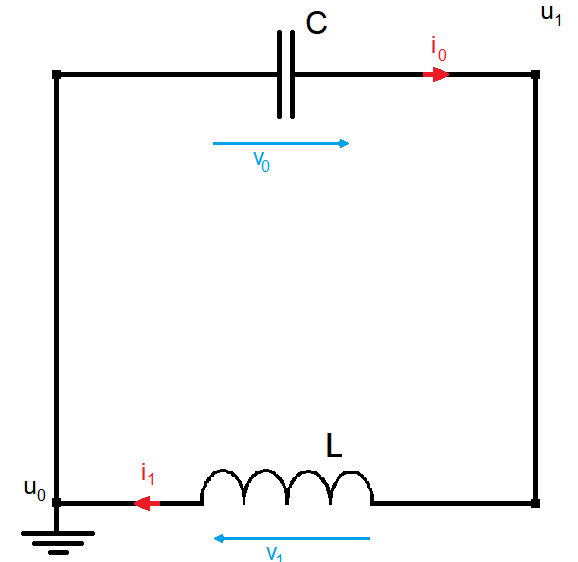
\includegraphics[width=\linewidth]{pictures/Example2_index0.png}
			\caption{LC-circuit}
			\label{fig: LC-circuit}
		\end{minipage}%
		\begin{minipage}{.5\textwidth}
			\centering
			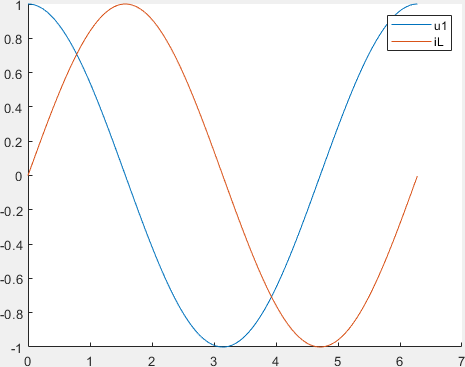
\includegraphics[width=\linewidth]{pictures/exact_solution_ex2.png}
			\caption{Exact solution for example 2.}
			\label{fig: Exact solution for example 2}
		\end{minipage}
	\end{figure}
	
	We again set $L=1$ and $C=1$. The resulting MNA-system for this example then reads
	
	\begin{displaymath}
		\begin{pmatrix}
			1 & 0 \\
			0 & 1 
		\end{pmatrix}
		*
		\begin{pmatrix}
			u_1' \\
			i_L'
		\end{pmatrix}
		+
		\begin{pmatrix}
			0 & 1 \\
			-1 & 0
		\end{pmatrix}
		*
		\begin{pmatrix}
			u_1 \\
			i_L
		\end{pmatrix}
		=
		\begin{pmatrix}
			0 \\
			0 
		\end{pmatrix}.
	\end{displaymath}
	
	When applying the BDF-k methods in Section \ref{sec:BDFk} and the trapezoidal rule in Section \ref{sec:Trapezoidal} to this problem, we can observe the maximal error $err(y) = \max\limits_{0 \leq n \leq N} | y(t_n) - y_n |$. The error is displayed in Table \ref{tab:error ex2}, where we again observe, that the errors reflect the predicted convergence rates.
		
	\begin{table}[H]
		\resizebox*{\textwidth}{!}{%
			\csvreader[tabular= | c || c c | c c | c c | c c | ,
			table head = \hline h & \multicolumn{2}{c|}{k = 1} & \multicolumn{2}{c|}{k = 2} & \multicolumn{2}{c|}{k = 3} & \multicolumn{2}{c|}{trapezoidal} \\
			& $err(u_1)$ & $err(i_l)$ & $err(u_1)$ & $err(i_l)$ & $err(u_1)$ & $err(i_l)$ & $err(u_1)$ & $err(i_l)$ \\
			\hline,
			late after line=\\\hline]
			{../Matlab/err_ex2.csv}{h=\h, oneu=\oneu, onei=\onei, twou=\twou, twoi=\twoi, threeu=\threeu, threei=\threei, trapu=\trapu, trapil=\trapil}
			{\h & \num{\oneu} & \num{\onei} & \num{\twou} & \num{\twoi} & \num{\threeu} & \num{\threei} & \num{\trapu} & \num{\trapil}}
		}
		\caption{Resulting errors for the BDF-k methods and the trapezoidal rule.}
		\label{tab:error ex2}
	\end{table}

\end{example2}
	


\begin{example3}[Numerical computation]
	
	In our last example we consider again the circuit given in Figure \ref{fig:num ex3}.
	\begin{figure}[H]
		\centering
		\begin{minipage}{.5\textwidth}
			\centering
			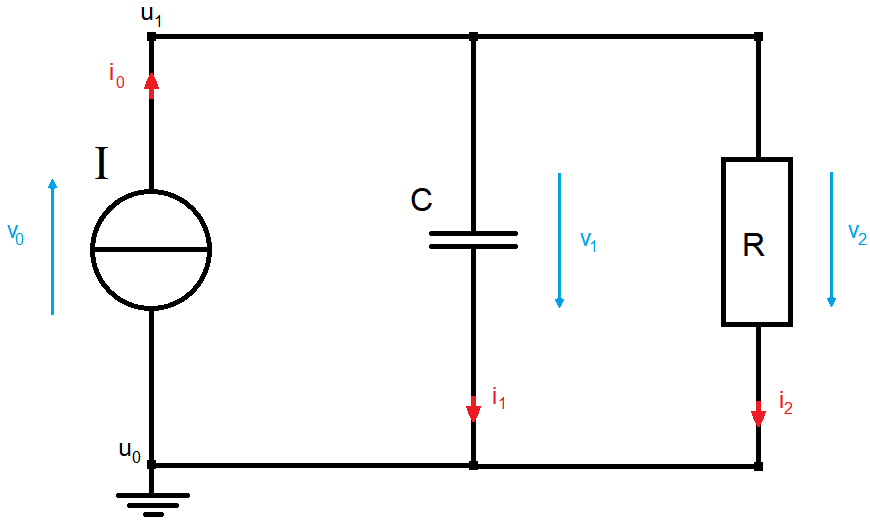
\includegraphics[width=\linewidth]{pictures/Example3.png}
			\caption{Current source with capacitor and resistor.}
			\label{fig:num ex3}
		\end{minipage}%
		\begin{minipage}{.5\textwidth}
			\centering
			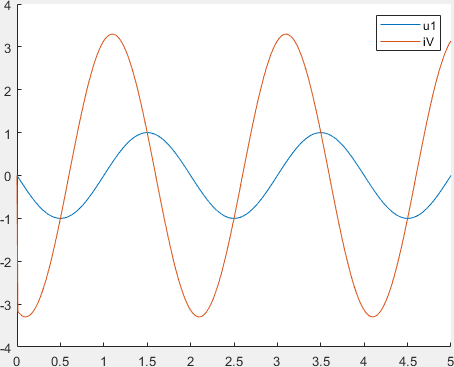
\includegraphics[width=\linewidth]{pictures/exact_solution_ex3.png}
			\caption{Exact solution for example 3.}
			\label{fig: Exact solution for example 3}
		\end{minipage}
	\end{figure}
	
	Setting $R=1$, $C=1$ and $v_{src} = sin(\pi t)$ the resulting system has the form
	\begin{displaymath}
			\begin{pmatrix}
			1 & 0 \\
			0 & 0 
		\end{pmatrix}
		*
		\begin{pmatrix}
			u_1' \\
			i_V'
		\end{pmatrix}
		+
		\begin{pmatrix}
			1 & -1 \\
			1 & 0
		\end{pmatrix}
		*
		\begin{pmatrix}
			u_1 \\
			i_V
		\end{pmatrix}
		=
		\begin{pmatrix}
			0 \\
			-sin(\pi t)
		\end{pmatrix}.
	\end{displaymath}
		
	With this we expect the potential and current to be given as illustrated in Figure \ref{fig: Exact solution for example 3}.

	The numerical methods result in errors displayed in Table \ref{tab:error ex3}. Due to the fact, that $u_1$ is again the same as $-v_{src}$, it is not of interest for our comparison of the errors, hence we omit $u_1$.
	
	\begin{table}[H]
		%\resizebox*{\textwidth}{!}{%
			\centering
			\csvreader[tabular= | c || c | c | c | c | ,
			table head = \hline h & {k = 1} & {k = 2} & {k = 3} & trapezoidal \\ %\multicolumn{1}{c|}{}
			& $err(i_V)$ & $err(i_V)$ & $err(i_V)$ & $err(i_V)$ \\
			\hline,
			late after line=\\\hline]
			{../Matlab/err_ex3.csv}{h=\h, oneu=\oneu, onei=\onei, twou=\twou, twoi=\twoi, threeu=\threeu, threei=\threei, trapu=\trapu, trapil=\trapil}
			{\h & \num{\onei} & \num{\twoi} & \num{\threei} & \num{\trapil}}
		%}
		\caption{Resulting errors for the BDF-k methods and the trapezoidal rule.}
		\label{tab:error ex3}
	\end{table}
	
	The errors rates are again within the expected range.
		
\end{example3}
	
\subsection{Results for the Gauss method}

	Observer that in the first example only the derivative of $u_2$ appears, thus $u_2$ is the differential variable while $u_1$ and $i_0$ are algebraic variables. For the second example both $u_1$ and $i_L$ are differential variables. In the third example $u_1$ is differential and $i_V$ is algebraic. We indicate this in Table \ref{tab:error gauss} by ``alg'' and by ``diff''.
	
	\begin{table}[H]
		\resizebox*{\textwidth}{!}{%
			\csvreader[tabular= | c || c c c | c c | c c |,
			table head = \hline h & \multicolumn{3}{c|}{example 1} & \multicolumn{2}{c|}{example 2} & \multicolumn{2}{c|}{example 3}\\
			& $err(u_1)$ (alg) & $err(u_2)$ (diff) & $err(i_0)$ (alg) & $err(u_1)$ (diff) & $err(i_L)$ (diff) & $err(u_1)$ (diff) & $err(i_V)$ (alg)\\
			\hline,
			late after line=\\\hline]
			{../Matlab/err_gauss.csv}{h=\h, oneu=\oneu, oneuu=\oneuu, onei=\onei, twou=\twou, twoi=\twoi, twoignore=\twoignore, threeu=\threeu, threei=\threei, threeignore=\threeignore}
			{\h  & \num{\oneu} & \num{\oneuu} & \num{\onei}  & \num{\twou} & \num{\twoi}  & \num{\threeu} & \num{\threei}}
		}
		\caption{Resulting errors for the Gauss method with one stage.}
		\label{tab:error gauss}
	\end{table}
	
	Comparing the table of errors \ref{tab:error gauss} with the table of convergence rates \ref{tab:convergence order Gauss} we observe that firstly the method converges as expected with approximately order $p=2$ for the ODE in example 2. In example 1 and in example 3 on the other hand we can observe different rates for the algebraic and the differential variables. In particular example 3, which has index $\nu = 2$ does not converge in its algebraic variables, in contrary, the error even grows.
%	\begin{center}
%		\begin{tabular}{ c || c c c | c c c | c c c | } 
%			h & \multicolumn{3}{c|}{k = 1} & \multicolumn{3}{c|}{k = 2} & \multicolumn{3}{c|}{k = 3} \\
%			& u1 & u2 & iL & u1 & u2 & iL & u1 & u2 & iL \\
%			\hline
%			& \multicolumn{3}{c|}{Error} & \multicolumn{3}{c|}{Error} & \multicolumn{3}{c|}{Error} \\
%			\hline
%			1 & number & number & number & number & number & number & number & number & number \\
%			0,1 & number & number & number & number & number & number & number & number & number \\
%			0,01 & number & number & number & number & number & number & number & number & number
%		\end{tabular}
%	\end{center}